\providecommand{\main}{.}
\documentclass[\main/main]{subfiles}
\setboolean{isMain}{false}

\begin{document}

\section{Fast Algorithm for Overlap}

As we stated in Theorem~\cite{thm:complexityStabilizerOverlap},
we can calculate the all overlap of the stabilizer states efficiently.
In this section, we will explain the algorithm in detail
and introduce some heuristics to improve the efficiency.

\subsection{Efficient Enumeration of Stabilizer States}

As we stated in the proposition~\ref{prop:originalStabilizerStateStandardForm},
there are the form of the stabilizer states.
Here, we will show a more efficient way to enumerate all the stabilizer states
by modifying the form slightly.
\begin{theorem}\label{thm:stabilizerStatesStandardForm}
  The form~\eqref{eq:stabilizerStateStandardForm}
  with the following conditions enumerates all the stabilizer states
  without any duplication or omission:
  \begin{quote}
    \begin{itemize}
      \item $Q$ is a upper triangular $\bbF_2^{k \times k}$ matrix.
      \item $R$ is a $\rank{k}$ $\bbF_2^{k \times (n-k)}$ rref (reduced row echelon form) matrix.
      \item $t$ belongs to the complement of the row space of $R$.
    \end{itemize}
  \end{quote}
\end{theorem}
\begin{proof}
  Main Ideas come from \cite{struchalinExperimentalEstimationQuantum2021b}.
  Firstly, we show that the mapping $\{(Q,c,R,t)\} \to \calS_n$ is injective.
  We can say that
  \begin{align*}
         & \left\{R_1 x + t_1 \;\middle|\; x \in \bbF_2^{n-k} \right\} = \left\{R_2 x + t_2 \;\middle|\; x \in \bbF_2^{n-k} \right\} \\
    \iff & \Im(R_1)=\Im(R_2) \land (t_2-t_1) \in \Im(R_1)                                                                            \\
    \iff & R_1 = R_2 \land t_1 = t_2.
  \end{align*}
  The last equivalence is due to the
  property of the rref matrix and the complement condition.
  Since $Q$ is a upper triangular matrix,
  we can uniquely determine $Q$ and $c$
  for given state $\ket{\phi}$.
  Thus, if two states are the same,
  then the corresponding $(Q,c,R,t)$ are also the same,
  which means that the mapping is injective.

  Next, we show that the mapping is surjective.
  Since the mapping is injective, we only have to show
  that the cardinality of the domain is equal to that of the codomain, i.e., $\abs{\calS_n}$.
  It is known that the number of $\rank k$ $\bbF_2^{k \times (n-k)}$ rref matrices is
  $\qBinom{n}{k}_2$, which is a q-binomial coefficient with $q=2$.
  Therefore, the number of $Q,c,R,t$ is
  $2^{k(k+1)/2},2^k,\qBinom{n}{k}_2,2^{n-k}$, respectively,
  and the total number of states is
  \begin{equation*}
    2^n + \sum_{k=1}^{n} 2^{k(k+1)/2} 2^k \qBinom{n}{k}_2 2^{n-k} \\
    = 2^n \sum_{k=0}^{n} \qBinom{n}{k}_2 2^{k(k+1)/2}               \\
    = 2^n \prod_{k=1}^{n} (2^k+1)
    = \abs{\calS_n}.
  \end{equation*}
  In the second last equation, we used the q-binomial theorem.
  Therefore, the mapping is surjective, which concludes the proof.
\end{proof}

In theorem~\ref{thm:stabilizerStatesStandardForm},
we used $\bbF_2$.
However, in the viewpoint of the dfs algorithm,
it is more practical to use $\{0,1\} \subset \bbZ$
and allow the term $c^\top x$ to be any integer.
Therefore, the following corollary is useful.
\begin{corollary}\label{cor:stabilizerStateStandardFormWithZ}
  In theorem~\ref{thm:stabilizerStatesStandardForm},
  We can substitute $\bbF_2$ with $\{0,1\} \subset \bbZ$.
\end{corollary}
\begin{proof}
  By changing $\bbF_2$ to $\{0,1\} \subset \bbZ$,
  the term $(-1)^{x^\top Q x}$ is invariant,
  and the term $i^{c^\top x}$ is multiplied by $-1$
  iff $p \equiv 2,3 \pmod 4$,
  where $p$ is the number of $i$ such that $c_i=1$ and $x_i=1$.
  Now, we consider the following form:
  \begin{equation}\label{eq:stabilizerStateStandardFormWithZ}
    \begin{dcases}
      \ket{\phi} \defeq \ket{t}                                                                            & \text{if $k=0$}, \\
      \ket{\phi} \defeq \frac{1}{2^{k/2}} \sum_{x=0}^{2^k-1}(-1)^{x^\top (Q+Q') x} i^{c^\top x}\ket{R x+t} & \text{if $k>0$},
    \end{dcases}
  \end{equation}
  where $Q \in \{0,1\}^{k \times k}, c \in \{0,1\}^k,
    R \in \{0,1\}^{k \times (n-k)}, t \in \{0,1\}^{n-k}, \Rank{R} = k$
  and $Q'_{ij} = 1$ iff $(i<j) \land (c_i=c_j=1)$.
  Now, if the pair $(Q,c,R,t)$ in~\eqref{eq:stabilizerStateStandardFormWithZ} is
  the same as that of the original form~\eqref{eq:stabilizerStateStandardForm},
  then the two states are representing the exactly same state
  since
  \begin{align*}
    (-1)^{x^\top Q' x}=(-1)^{\binom{p}{2}}=
    \begin{cases}
      1  & \text{if $p \equiv 0,1 \pmod 4$}, \\
      -1 & \text{if $p \equiv 2,3 \pmod 4$}.
    \end{cases}
  \end{align*}
  Therefore, by identifying the $Q+Q'$ in $\bbZ$ with new $Q''$ in $\bbF_2$,
  we can conclude the proof.
\end{proof}

\subsection{Calculating the Overlap}

\begin{figure}[htbp]
  \centering
  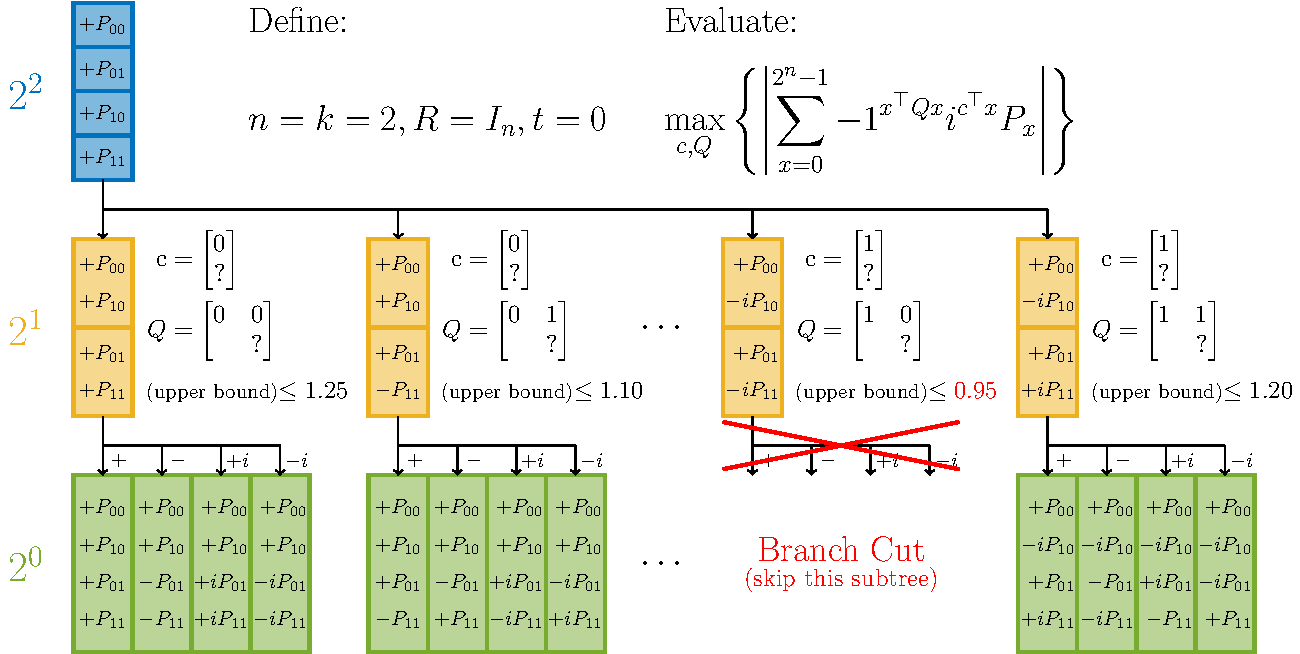
\includegraphics[width=\columnwidth]{imgs/dfs.pdf}
  \caption{
    The visualization of the DFS algorithm.
    The DFS algorithm is a recursive algorithm
    that calculates the overlap of the stabilizer states
    by recursively calculating the overlap of the substates.
    The algorithm is efficient since the overlap of the substates
    can be calculated with very small computational cost.
  }
  \label{fig:dfs}
\end{figure}

Thanks to the corollary \ref{cor:stabilizerStateStandardFormWithZ},
we can prove the following theorem.
\begin{theorem}
  Fix $k,R,t$ in the standard form \eqref{eq:stabilizerStateStandardForm}.
  Then, we can compute the overlap $\braket{\phi}{\psi}$ efficiently.
\end{theorem}
\begin{proof}
  We only consider the case $k>0,R=0,t=0$ for the simplicity.
  Other cases are trivial or can be reduced to this case.
  Define $x \defeq \begin{bmatrix}
      x_0 \\
      \overline{x}
    \end{bmatrix}$,
  $c \defeq \begin{bmatrix}
      c_0 \\
      \overline{c}
    \end{bmatrix}$, and
  $Q \defeq \begin{bmatrix}
      Q_{00} & Q_{0}^\top   \\
      0      & \overline{Q}
    \end{bmatrix}$
  ($x_0,c_0$ and $Q_{00}$ are all in $\{0,1\}$).
  Since
  $x^\top Q x = x_0 (Q_{00}+Q_0^\top \overline{x}) + \overline{x}^\top \overline{Q} \overline{x}$
  and
  $c^\top x = c_0 x_0 + \overline{c}^\top \overline{x}$,
  we can rewrite the state as
  \begin{align*}
    \ket{\phi} & = \sum_{x=0}^{2^k-1} (-1)^{x^\top Q x} i^{c^\top x} \ket{x}                                                                                   \\
               & = \sum_{\overline{x}=0}^{2^{k-1}-1} (-1)^{\overline{x}^\top \overline{Q} \overline{x}} i^{\overline{c}^\top \overline{x}}
    \qty(\ket{2\overline{x}} + (-1)^{Q_{00}+Q_0^\top \overline{x}} i^{c_0} \ket{2\overline{x}+1})                                                              \\
               & = \sum_{\overline{x}=0}^{2^{k-1}-1} (-1)^{\overline{x}^\top \overline{Q} \overline{x}} i^{\overline{c}^\top \overline{x}} \ket{\overline{x}'}
  \end{align*}
  by defining $\ket{\overline{x}'} \defeq \ket{2\overline{x}} + (-1)^{Q_{00}+Q_0^\top \overline{x}} i^{c_0} \ket{2\overline{x}+1}$.
  (Question: Is it natural to equate integer $2\overline{x}+1$ to the vector $\begin{bmatrix} 1 \\ \overline{x} \end{bmatrix}$?)

  Thus, we can compute the overlap recursively
  with very small computational cost per each step.
  This leads to the efficient calculation of the overlaps,
  which concludes the proof.
\end{proof}

\subsection{Branch Cut For The DFS}

In this section, we will explain the branch cut methods used in the dfs search.
Firstly, please recall that we are maximizing the following:
\begin{equation*}
  \max_{c,Q} \qty{ \abs{\sum_{x=0}^{2^n-1} -1^{x^\top Q x} i^{c^\top x} P_x} }
\end{equation*}

This value can easily evaluate as the following:
\begin{equation*}
  \max_{c,Q} \qty{ \abs{\sum_{x=0}^{2^n-1} -1^{x^\top Q x} i^{c^\top x} P_x} }
  \leq \max_{c,Q} \qty{ \sum_{x=0}^{2^n-1} \abs{-1^{x^\top Q x} i^{c^\top x} P_x} }
  = \sum_{x=0}^{2^n-1} \abs{P_x}
\end{equation*}

However, since each coefficient takes only $1, -1, i$ or $-i$,
we can obtain more tight bound by
\begin{equation}\label{eq:branchCutNewProblemDefinition}
  \max_{c,Q} \qty{ \abs{\sum_{x=0}^{2^n-1} -1^{x^\top Q x} i^{c^\top x} P_x} }
  \leq \max_{c,Q} \qty{ \abs{\sum_{x=0}^{2^n-1} i^{c_x} P_x} }
\end{equation}
where $c_x \in \qty{0, 1, 2, 3}$ is the independent variable for each $x$.
Let $\calP \defeq \sum_{x=0}^{2^n-1} i^{c_x^*} P_x$ be
the one of optimal solutions for the problem~\eqref{eq:branchCutNewProblemDefinition}.
Then, without loss of generality,
we can assume that $\frac{\pi}{2} \leq \arg \calP < \frac{3\pi}{2}$.
Additionally, by sorting and relabeling we can also assume that
$0 \leq \arg{(P_0)} \leq \arg{(P_1)} \leq \dots \leq \arg{(P_{2^n-1})} < \pi/2$.
Suppose we fix the answer $\calP$.
If all $c_x$ satisfies $\arg{(\calP)} - \pi/4 \leq \arg{\qty(i^{c_x} P_x)} < \arg{(\calP)} + \pi/4$,
then $c_x$ is optimal for the fixed $\calP$.
Therefore, we can justify the following Algorithm \ref{alg:branchCut}
by moving $\arg(\calP)$ in the range of $[\pi/2, 3\pi/2)$.
Also refer to the figure~\ref{fig:argsort} for the visualization of this algorithm.
The time complexity of this algorithm is $O(n2^n)$ due to the sorting.

\begin{algorithm}
  \caption{Branch Cut Algorithm}
  \label{alg:branchCut}
  \KwIn{The coefficients $P_x$ which are sorted by the argument}
  \KwOut{The answer for the problem~\eqref{eq:branchCutNewProblemDefinition}}
  $\mathrm{ans} \leftarrow 0, \quad c_x \leftarrow 0 \quad \text{for all } x$\;
  \For{$x \leftarrow 0$ \KwTo $2^n - 1$}{
    $\mathrm{ans} \leftarrow \max\qty(\mathrm{ans}, \abs{\sum_{x=0}^{2^n-1} i^{c_x} P_x})$\;
    $c_x \leftarrow c_x + 1$\;
  }
  \KwRet{$\mathrm{ans}$}
\end{algorithm}

\begin{figure}[htbp]
  \centering
  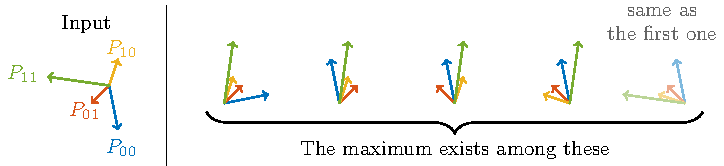
\includegraphics[width=\columnwidth]{imgs/argsort.pdf}
  \caption{
    The visualization of Algorithm \ref{alg:branchCut}.
    Suppose that $n=2$ and $P_x$ are represented as the vectors in the complex plane
    (for example, $P_{00} = 1-5i$) by the left figure.
    Then, by sorting and iterating the loop in Algorithm \ref{alg:branchCut},
    we can obtain $2^n$ patterns of the coefficients $c_x$ as the right figure.
    The maximum of for the problem \eqref{eq:branchCutNewProblemDefinition}
    exists among these $2^n$ patterns.
  }
  \label{fig:argsort}
\end{figure}

\end{document}
